\documentclass[11pt,a4paper]{article}
\usepackage[T1]{fontenc}\usepackage{lmodern}\usepackage[margin=2.2cm]{geometry}\usepackage{microtype}
\usepackage{booktabs}\usepackage{tabularx}\usepackage{longtable}\usepackage{array}\usepackage{float}
\usepackage{caption}\usepackage{enumitem}\usepackage{xcolor}\usepackage{amsmath}
\usepackage{pgfplots}\pgfplotsset{compat=1.18}\usepgfplotslibrary{groupplots}
\usepackage[colorlinks=true,linkcolor=blue!50!black,urlcolor=blue!50!black]{hyperref}
\definecolor{seriesA}{HTML}{2A78D6}\definecolor{seriesB}{HTML}{EB6834}
\captionsetup{font=small,labelfont=bf}\setlist{itemsep=2pt,topsep=4pt}\setlength{\emergencystretch}{3em}
\newcolumntype{Y}{>{\raggedright\arraybackslash}X}
\pgfplotsset{every axis/.append style={axis line style={draw=black!40}, tick style={draw=black!40},
  ymajorgrids, grid style={draw=black!12}, legend style={draw=none, font=\small}}}
\title{\textbf{Hybrid Video Provenance Framework (HVPF)}\\[3pt]\large Phase 2 Results}
\author{Talha Aslam\\ MS Thesis}
\date{12 October 2026}
\begin{document}\maketitle
\begin{abstract}\noindent
This report presents the Phase 2 results of the HVPF pipeline: a three-class decision
(organic / manipulated / synthetic) for video clips, compared with the conventional PRNU method (PCE rule).
Phase 2 extends Phase 1 with the full Video-ACID dataset, FloreView as an unseen-camera test set,
additional genuine re-encodes, and WhatsApp-/YouTube-like copies of genuine, attacked and AI-generated clips.
All numbers are generated directly from the result files.
\end{abstract}
\section{Key results}\begin{itemize}
\item \textbf{Best model:} XGBoost reaches PVA 0.785, macro F1 0.792 and authentic-vs-not AUC 0.899 (EER 0.193) in 5-fold cross-validation on cameras never seen in training, against AUC 0.635 (EER 0.401) for the conventional PCE rule (RQ3).
\item \textbf{Honest benchmark:} Phase 1 recognised 99\% of genuine WhatsApp copies, but only because no fake clip was WhatsApp-compressed. With WhatsApp-like copies of fakes the rate is 57\%, which is why Phase 2 scores are lower.
\item \textbf{Genuine re-encodes:} in the encoder-controlled setup, XGBoost macro F1 rose from 0.703 (Phase 1) to 0.770.
\item \textbf{5 vs 10 frames:} 10 frames looks better on the full data, but only because sequence models learn the clip length (attacked clips have 30 frames, ACID and AI clips about 6). With clips of equal length the two windows perform the same (Table~\ref{tab:window}); 5 frames is the main setting.
\item \textbf{Unseen cameras:} on FloreView (45 cameras, never trained on) genuine videos of phones with a usable PRNU are mostly recognised, but phones whose stabilisation removes the PRNU are the hardest case (Table~\ref{tab:cross}).
\item \textbf{Features (RQ1):} removing Noiseprint statistics costs the most, followed by PRNU and TSNCS; FFT and residual moments add almost nothing (Figure~\ref{fig:ablation}).
\end{itemize}
\section{Data and protocol}
The evaluation uses 24,599 clips. Model inputs come from the first five I-frames of each clip. Results are averaged over five grouped cross-validation folds: no camera model is in both training and test. \emph{Realistic} uses all clips; \emph{encoder-controlled} uses only clips encoded by our libx264 pipeline (genuine re-encodes, attacks, AI clips), so encoder traces cannot separate the classes. \emph{Cross-dataset} is FloreView (genuine) plus GenBuster (unseen AI generators), tested with the fixed-split models.
\begin{table}[H]\centering\small\caption{Clips per class and source.}\begin{tabular}{llr}\toprule Class & Source & Clips \\\midrule
manipulated & VISION-attack & 7,200 \\
organic & ACID & 4,380 \\
organic & ACID-attack & 3,168 \\
organic & FloreView & 1,716 \\
organic & VISION & 1,259 \\
organic & VISION-attack & 2,400 \\
synthetic & GenBuster & 1,800 \\
synthetic & GenVidBench & 2,676 \\
\bottomrule\end{tabular}\end{table}
\section{Main results}
\begin{table}[H]\centering\small\caption{Realistic setup, 5-fold cross-validation (mean $\pm$ std over folds), 5 frames. PVA = share of clips assigned to their true provenance class; AUC/EER for genuine vs not genuine.}\label{tab:main}\begin{tabular}{lccccc}\toprule Model & PVA & Macro F1 & AUC (3-class) & AUC genuine vs not & EER \\\midrule
PCE rule & -- & -- & -- & 0.635 & 0.401 \\
SVM & 0.761 $\pm$ 0.022 & 0.770 $\pm$ 0.028 & 0.897 & 0.867 & 0.215 \\
XGBoost & 0.785 $\pm$ 0.027 & 0.792 $\pm$ 0.028 & 0.923 & 0.899 & 0.193 \\
GRU & 0.774 $\pm$ 0.020 & 0.785 $\pm$ 0.021 & 0.917 & 0.891 & 0.205 \\
1D-CNN & 0.765 $\pm$ 0.036 & 0.774 $\pm$ 0.042 & 0.909 & 0.880 & 0.211 \\
Transformer & 0.761 $\pm$ 0.018 & 0.775 $\pm$ 0.016 & 0.908 & 0.880 & 0.213 \\
\bottomrule\end{tabular}\end{table}
\begin{table}[H]\centering\small\caption{Encoder-controlled setup (5-fold) and cross-dataset test (FloreView + GenBuster), 5 frames.}\begin{tabular}{lcccccc}\toprule & \multicolumn{3}{c}{Encoder-controlled} & \multicolumn{3}{c}{Cross-dataset} \\\cmidrule(lr){2-4}\cmidrule(lr){5-7} Model & PVA (\%) & Macro F1 & AUC & PVA (\%) & Macro F1 & AUC \\\midrule
PCE rule & -- & -- & 0.598 & -- & -- & 0.654 \\
SVM & 74 & 0.757 & 0.841 & 48 & 0.583 & 0.729 \\
XGBoost & 75 & 0.770 & 0.867 & 58 & 0.682 & 0.886 \\
GRU & 74 & 0.765 & 0.857 & 60 & 0.692 & 0.842 \\
1D-CNN & 74 & 0.757 & 0.854 & 56 & 0.672 & 0.848 \\
Transformer & 73 & 0.757 & 0.848 & 52 & 0.653 & 0.829 \\
\bottomrule\end{tabular}\end{table}
\begin{table}[H]\centering\small\caption{Phase 1 vs Phase 2 (realistic, 5-fold, 5 frames). Phase 2 is harder by design: fakes also appear as platform-like copies and there are four times more genuine ACID clips.}\begin{tabular}{lcccccc}\toprule & \multicolumn{2}{c}{PVA (\%)} & \multicolumn{2}{c}{Macro F1} & \multicolumn{2}{c}{AUC genuine vs not} \\\cmidrule(lr){2-3}\cmidrule(lr){4-5}\cmidrule(lr){6-7} Model & Phase 1 & Phase 2 & Phase 1 & Phase 2 & Phase 1 & Phase 2 \\\midrule
PCE rule & -- & -- & -- & -- & 0.570 & 0.635 \\
XGBoost & 83 & 78 & 0.842 & 0.792 & 0.937 & 0.899 \\
GRU & 84 & 77 & 0.852 & 0.785 & 0.930 & 0.891 \\
Transformer & 82 & 76 & 0.830 & 0.775 & 0.916 & 0.880 \\
\bottomrule\end{tabular}\end{table}
\section{5 vs 10 frames}
The length-matched columns use only clips with at least 10 I-frames (2,491 test clips per fold), so both windows see the same clips and the clip length carries no information.
\begin{table}[H]\centering\small\caption{Effect of the frame window (realistic, 5-fold).}\label{tab:window}\begin{tabular}{lcccccccc}\toprule & \multicolumn{4}{c}{All clips} & \multicolumn{4}{c}{Length-matched ($\geq$ 10 frames)} \\\cmidrule(lr){2-5}\cmidrule(lr){6-9} & \multicolumn{2}{c}{5 frames} & \multicolumn{2}{c}{10 frames} & \multicolumn{2}{c}{5 frames} & \multicolumn{2}{c}{10 frames} \\Model & PVA & AUC & PVA & AUC & PVA & AUC & PVA & AUC \\\midrule
XGBoost & 78 & 0.899 & 81 & 0.915 & 73 & 0.831 & 73 & 0.845 \\
GRU & 77 & 0.891 & 82 & 0.926 & 71 & 0.814 & 71 & 0.817 \\
1D-CNN & 77 & 0.880 & 83 & 0.930 & 68 & 0.790 & 69 & 0.807 \\
Transformer & 76 & 0.880 & 83 & 0.929 & 70 & 0.796 & 70 & 0.800 \\
\bottomrule\end{tabular}\end{table}
\section{Results per condition (RQ2)}
Share of clips assigned to their true class (\%), realistic setup, 5-fold, 5 frames. Values below 70\% are in bold. The PCE rule only decides genuine vs not genuine: its high rates on attacks and AI clips come with rejecting most genuine clips.
{\small\setlength{\tabcolsep}{4pt}\begin{longtable}{p{7.2cm}rrrrrrr}
\caption{Detection rate per condition.}\label{tab:cond}\\\toprule Condition & $n$ & PCE & SVM & XGB & GRU & CNN & Transf. \\\endfirsthead\toprule Condition & $n$ & PCE & SVM & XGB & GRU & CNN & Transf. \\\endhead\bottomrule\endfoot
\midrule\multicolumn{8}{l}{\textbf{Genuine (organic)}} \\
ACID native & 4380 & 36 & 91 & 94 & 93 & 92 & 92 \\
VISION native & 425 & 39 & 78 & 88 & 83 & 83 & 79 \\
VISION real WhatsApp copy & 423 & 5 & \textbf{47} & \textbf{57} & \textbf{46} & \textbf{47} & \textbf{35} \\
VISION real YouTube copy & 411 & 10 & \textbf{57} & \textbf{68} & \textbf{64} & \textbf{62} & \textbf{63} \\
ACID genuine re-encode, CRF 18 & 528 & 28 & 88 & 92 & 92 & 88 & 89 \\
ACID genuine re-encode, CRF 20 & 528 & 25 & 86 & 89 & 88 & 84 & 86 \\
ACID genuine re-encode, CRF 20 + WA-like & 528 & 0 & \textbf{52} & \textbf{63} & \textbf{38} & \textbf{51} & \textbf{29} \\
ACID genuine re-encode, CRF 20 + YT-like & 528 & 8 & 81 & 86 & 84 & 77 & 81 \\
ACID genuine re-encode, CRF 23 & 528 & 20 & 84 & 86 & 85 & 81 & 85 \\
ACID genuine re-encode, CRF 28 & 528 & 9 & 85 & 86 & 89 & 83 & 85 \\
VISION genuine re-encode, CRF 18 & 400 & 24 & \textbf{67} & 74 & \textbf{69} & 70 & \textbf{67} \\
VISION genuine re-encode, CRF 20 & 400 & 21 & \textbf{55} & \textbf{63} & \textbf{59} & \textbf{59} & \textbf{58} \\
VISION genuine re-encode, CRF 20 + WA-like & 400 & 2 & \textbf{25} & \textbf{34} & \textbf{28} & \textbf{29} & \textbf{21} \\
VISION genuine re-encode, CRF 20 + YT-like & 400 & 10 & \textbf{40} & \textbf{48} & \textbf{49} & \textbf{47} & \textbf{45} \\
VISION genuine re-encode, CRF 23 & 400 & 17 & \textbf{48} & \textbf{62} & \textbf{52} & \textbf{52} & \textbf{50} \\
VISION genuine re-encode, CRF 28 & 400 & 9 & \textbf{43} & \textbf{53} & \textbf{53} & \textbf{50} & \textbf{45} \\
\midrule\multicolumn{8}{l}{\textbf{Manipulated}} \\
denoise\_a1 & 400 & 84 & \textbf{66} & \textbf{57} & \textbf{68} & \textbf{63} & \textbf{66} \\
denoise\_a2 & 400 & 84 & 78 & 70 & 77 & 75 & 76 \\
denoise\_a2 + WA-like & 400 & 99 & 72 & \textbf{68} & \textbf{67} & \textbf{67} & 77 \\
denoise\_a2 + YT-like & 400 & 95 & \textbf{68} & \textbf{63} & \textbf{67} & 70 & 71 \\
denoise\_a4 & 400 & 88 & 83 & 79 & 82 & 81 & 84 \\
injection\_a0.25 & 400 & 83 & 70 & \textbf{67} & \textbf{68} & \textbf{69} & \textbf{66} \\
injection\_a0.5 & 400 & 30 & 78 & 83 & 82 & 77 & 80 \\
injection\_a0.5 + WA-like & 400 & 98 & 74 & 70 & 73 & \textbf{68} & 79 \\
injection\_a0.5 + YT-like & 400 & 74 & 73 & \textbf{68} & 71 & 71 & 70 \\
injection\_a1 & 400 & 2 & 92 & 98 & 96 & 93 & 96 \\
removal\_a0.25 & 400 & 87 & \textbf{51} & \textbf{44} & \textbf{49} & \textbf{48} & \textbf{47} \\
removal\_a0.5 & 400 & 96 & \textbf{66} & 75 & 73 & 73 & 73 \\
removal\_a0.5 + WA-like & 400 & 100 & 70 & \textbf{66} & \textbf{68} & \textbf{64} & 75 \\
removal\_a0.5 + YT-like & 400 & 98 & \textbf{68} & \textbf{65} & \textbf{64} & \textbf{64} & \textbf{65} \\
removal\_a1 & 400 & 100 & 86 & 94 & 95 & 95 & 94 \\
removal\_opt & 400 & 99 & \textbf{62} & \textbf{61} & \textbf{64} & \textbf{66} & \textbf{65} \\
removal\_opt + WA-like & 400 & 100 & 73 & \textbf{66} & \textbf{68} & \textbf{66} & 74 \\
removal\_opt + YT-like & 400 & 100 & \textbf{62} & \textbf{56} & \textbf{58} & \textbf{60} & \textbf{60} \\
\midrule\multicolumn{8}{l}{\textbf{AI-generated (synthetic)}} \\
CogVideo & 294 & 100 & 97 & 98 & 98 & 96 & 97 \\
CogVideo + WA-like & 294 & 100 & 94 & 98 & 98 & 96 & 97 \\
CogVideo + YT-like & 294 & 100 & 95 & 98 & 97 & 95 & 95 \\
Kling & 266 & 100 & 89 & 91 & 89 & 85 & 85 \\
Kling + WA-like & 266 & 100 & 90 & 91 & 91 & 93 & 86 \\
Kling + YT-like & 266 & 100 & 89 & 87 & 88 & 79 & 76 \\
OpenSora & 267 & 100 & 96 & 98 & 98 & 98 & 97 \\
OpenSora + WA-like & 267 & 100 & 97 & 100 & 100 & 99 & 99 \\
OpenSora + YT-like & 267 & 100 & 98 & 100 & 100 & 100 & 100 \\
Sora & 49 & 100 & \textbf{49} & \textbf{37} & \textbf{43} & \textbf{37} & \textbf{37} \\
Sora + WA-like & 49 & 100 & \textbf{51} & \textbf{47} & \textbf{57} & \textbf{41} & \textbf{37} \\
Sora + YT-like & 49 & 100 & \textbf{59} & \textbf{55} & \textbf{55} & \textbf{41} & \textbf{51} \\
\end{longtable}}
\begin{figure}[H]\centering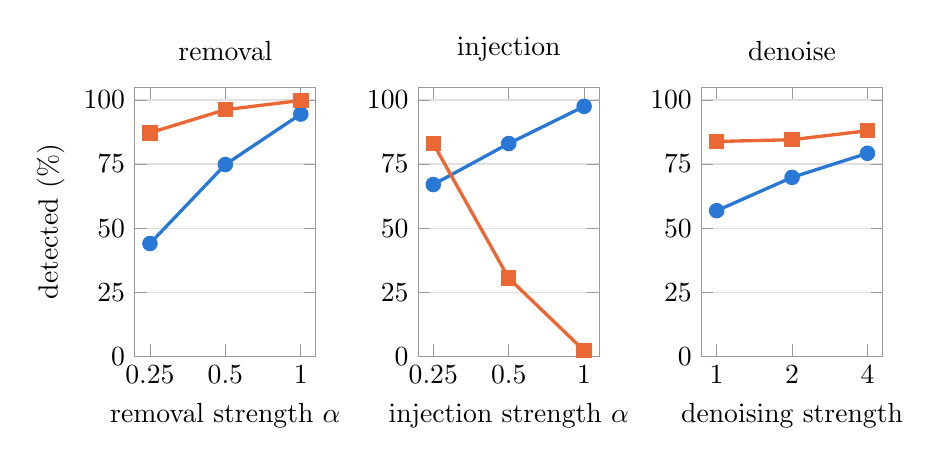
\begin{tikzpicture}\begin{groupplot}[group style={group size=3 by 1, horizontal sep=1.3cm},width=0.32\linewidth, height=5cm, ymin=0, ymax=105, ytick={0,25,50,75,100}]
\nextgroupplot[title={removal}, xlabel={removal strength $\alpha$}, xmode=log, log basis x=2, xtick={0.25,0.5,1}, xticklabels={0.25,0.5,1}, ylabel={detected (\%)}, legend to name=strengthlegend, legend columns=2]
\addplot[color=seriesA, mark=*, mark size=2.2pt, line width=1.2pt] coordinates {(0.25,44.0) (0.5,74.8) (1,94.5)};
\addplot[color=seriesB, mark=square*, mark size=2.2pt, line width=1.2pt] coordinates {(0.25,87.2) (0.5,96.2) (1,99.8)};
\legend{XGBoost, PCE rule}
\nextgroupplot[title={injection}, xlabel={injection strength $\alpha$}, xmode=log, log basis x=2, xtick={0.25,0.5,1}, xticklabels={0.25,0.5,1}]
\addplot[color=seriesA, mark=*, mark size=2.2pt, line width=1.2pt] coordinates {(0.25,67.0) (0.5,83.0) (1,97.5)};
\addplot[color=seriesB, mark=square*, mark size=2.2pt, line width=1.2pt] coordinates {(0.25,83.0) (0.5,30.5) (1,2.2)};
\nextgroupplot[title={denoise}, xlabel={denoising strength}, xmode=log, log basis x=2, xtick={1,2,4}, xticklabels={1,2,4}]
\addplot[color=seriesA, mark=*, mark size=2.2pt, line width=1.2pt] coordinates {(1,56.8) (2,69.8) (4,79.2)};
\addplot[color=seriesB, mark=square*, mark size=2.2pt, line width=1.2pt] coordinates {(1,83.8) (2,84.5) (4,88.0)};
\end{groupplot}\end{tikzpicture}\\[2pt]\ref{strengthlegend}\caption{Attack strength vs detection (VISION attacks, realistic, 5-fold). The PCE rule ``detects'' removal only because low PCE is its sign of non-genuine; it misses injection, where the victim's fingerprint is matched.}\label{fig:strength}\end{figure}
\section{Cross-dataset test}
FloreView cameras are split by their PRNU baseline: 10 of 45 cameras have a usable video PRNU (attribution $\geq$ 50\%); the others are modern phones whose stabilisation removes it.
\begin{table}[H]\centering\small\caption{Cross-dataset detection rate (\%), models trained on VISION + ACID + GenVidBench (fixed split).}\label{tab:cross}\begin{tabular}{lrrrrrrr}\toprule Condition & $n$ & PCE & SVM & XGB & GRU & CNN & Transf. \\\midrule
FloreView genuine, PRNU removed (stabilised) & 1361 & 0 & 29 & 44 & 51 & 44 & 38 \\
FloreView genuine, PRNU usable & 355 & 62 & 70 & 78 & 79 & 69 & 80 \\
GenBuster AI & 616 & 100 & 68 & 74 & 74 & 71 & 62 \\
GenBuster AI + WA-like & 616 & 100 & 43 & 43 & 49 & 47 & 45 \\
GenBuster AI + YT-like & 616 & 100 & 65 & 76 & 67 & 70 & 64 \\
\bottomrule\end{tabular}\end{table}
\section{Feature ablation (RQ1)}
\begin{figure}[H]\centering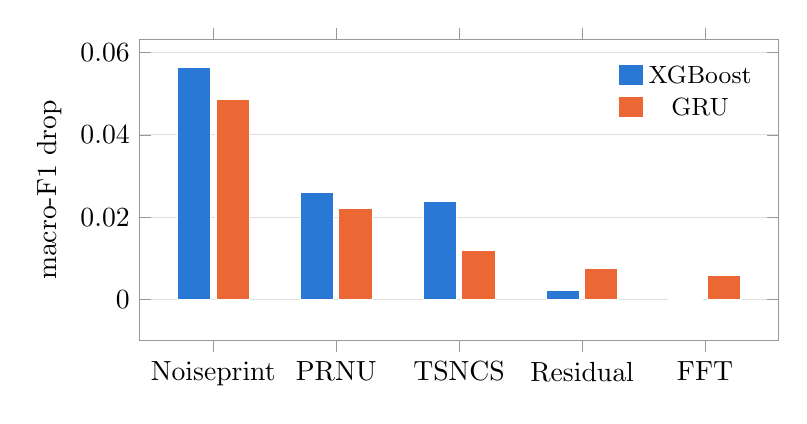
\begin{tikzpicture}\begin{axis}[ybar, bar width=12pt, width=0.8\linewidth, height=5.4cm,symbolic x coords={Noiseprint,PRNU,TSNCS,Residual,FFT}, xtick=data, ymin=-0.01, ylabel={macro-F1 drop}, enlarge x limits=0.15,scaled y ticks=false, yticklabel style={/pgf/number format/fixed, /pgf/number format/precision=2},legend style={at={(0.98,0.95)}, anchor=north east}, legend image code/.code={\draw[#1, draw=none] (0cm,-0.1cm) rectangle (0.3cm,0.15cm);}]
\addplot[fill=seriesA, draw=white] coordinates {(Noiseprint,0.0565) (PRNU,0.0259) (TSNCS,0.0237) (Residual,0.0022) (FFT,-0.0003)};
\addplot[fill=seriesB, draw=white] coordinates {(Noiseprint,0.0486) (PRNU,0.0221) (TSNCS,0.0119) (Residual,0.0075) (FFT,0.0057)};
\legend{XGBoost, GRU}\end{axis}\end{tikzpicture}\caption{Drop in macro F1 when one feature group is removed (realistic, 5-fold, 5 frames). Larger = more important.}\label{fig:ablation}\end{figure}
\begin{table}[H]\centering\small\caption{Macro-F1 drop per feature group and model (5-fold, 5 frames).}\begin{tabular}{llccccc}\toprule Setup & Removed group & SVM & XGB & GRU & CNN & Transf. \\\midrule
realistic & Noiseprint & 0.053 & 0.057 & 0.049 & 0.043 & 0.054 \\
realistic & PRNU & 0.021 & 0.026 & 0.022 & 0.009 & 0.016 \\
realistic & TSNCS & 0.012 & 0.024 & 0.012 & 0.016 & 0.018 \\
realistic & Residual & 0.002 & 0.002 & 0.008 & -0.004 & 0.002 \\
realistic & FFT & -0.001 & -0.000 & 0.006 & -0.003 & 0.003 \\
controlled & Noiseprint & 0.054 & 0.045 & 0.054 & 0.047 & 0.043 \\
controlled & PRNU & 0.031 & 0.033 & 0.025 & 0.020 & 0.017 \\
controlled & TSNCS & 0.014 & 0.024 & 0.013 & 0.011 & 0.002 \\
controlled & Residual & 0.009 & 0.004 & 0.001 & -0.008 & -0.006 \\
controlled & FFT & -0.003 & 0.002 & -0.001 & 0.005 & 0.005 \\
\bottomrule\end{tabular}\end{table}
\section{Comparison with the base papers}
The base papers solve related but different tasks, so each is compared on its own terms. Literature values are taken from the papers as reported; protocols differ (noted per table).
\subsection{Camera identification: PDC-ViT (Elharrouss et al.~2025)}
PDC-ViT is a learned camera-identification model (80/20 train-test split, every camera seen in training). The closest component of HVPF is the training-free PRNU baseline (Step 4): fingerprints from flat videos, tested on natural videos, closed-set over all cameras of the dataset; verification at PCE$_0>60$.
\begin{table}[H]\centering\small\caption{Camera identification. Accuracy = closed-set attribution; FNR/FPR = verification.}\setlength{\tabcolsep}{4pt}\begin{tabular}{llrrrr}\toprule Method & Dataset (cameras) & Accuracy (\%) & FNR (\%) & FPR (\%) & EER (\%) \\\midrule
PDC-ViT \cite{pdcvit} & VISION (35) & 94.30 & -- & -- & -- \\
HVPF PRNU & VISION (35) & 73.4 & 36.2 & 0.00 & 18.3 \\
HVPF PRNU & VISION (21 non-stabilised) & 100.0 & -- & -- & -- \\
\midrule PRNU \cite{pdcvit} & Video-ACID + WA (26) & -- & 41.9 & 3.6 & -- \\
WA-PRNU \cite{pdcvit} & Video-ACID + WA (26) & -- & 28.06 & 2.8 & -- \\
PDC-ViT \cite{pdcvit} & Video-ACID + WA (26) & 74.77 & 23.4 & 0.92 & -- \\
HVPF PRNU & Video-ACID (44) & 59.1 & 59.6 & 0.00 & 25.5 \\
\midrule HVPF PRNU & FloreView (45) & 26.2 & 80.8 & 0.00 & 38.8 \\
\bottomrule\end{tabular}\end{table}
PRNU matching needs no training and is perfect on non-stabilised VISION cameras, above PDC-ViT; electronic stabilisation is what lowers the all-camera figures. Our verification threshold is strict (FPR 0\%), so FNR is higher than PDC-ViT's (FPR 0.92\%); the EER gives a threshold-free view. PDC-ViT was not tested on manipulated or synthetic video, and no base paper uses FloreView.
\subsection{PRNU-transfer attack: Khan et al.~2025}
Khan et al.\ inject a camera's PRNU into images from another camera or from AI generators and report that 85.5\% of them pass source verification (images only). Our injection attack is the same attack on video. The compromise rate is the share of injected clips accepted as genuine: by the PCE rule if the victim's PCE$_0$ exceeds 60, by a model if it predicts \emph{organic} (realistic, 5-fold, 5 frames).
\begin{table}[H]\centering\small\caption{Compromise rate of PRNU injection (\%, lower is better for the defender).}\begin{tabular}{lrrrrrr}\toprule & \multicolumn{3}{c}{Injection strength $\alpha$} & \multicolumn{2}{c}{$\alpha$=0.5, re-shared} & \\\cmidrule(lr){2-4}\cmidrule(lr){5-6} Detector & 0.25 & 0.5 & 1 & WA-like & YT-like & All \\\midrule
Khan et al.~2025 \cite{khan2025}, images & \multicolumn{5}{c}{--} & 85.5 \\\midrule
PCE rule & 17 & 70 & 98 & 2 & 26 & 42 \\
SVM & 26 & 22 & 8 & 20 & 25 & 20 \\
XGBoost & 31 & 17 & 2 & 26 & 30 & 21 \\
GRU & 30 & 18 & 4 & 21 & 27 & 20 \\
1D-CNN & 30 & 23 & 7 & 26 & 28 & 23 \\
Transformer & 32 & 20 & 4 & 18 & 29 & 20 \\
\bottomrule\end{tabular}\end{table}
A full-strength injection fools the PCE rule in 98\% of the clips, in line with Khan et al.; the best model lets through only 2.5\%. Weak injections ($\alpha$=0.25) rarely fool PCE but are also harder for the models to spot.
\subsection{Low false-positive operation: Bao et al.~2024}
Bao et al.\ detect frame deletion (a different manipulation) from inter-frame noise consistency, the idea behind TSNCS, and stress performance at low false-positive rates; their results are given as ROC curves only. Table~\ref{tab:lowfpr} reports HVPF at the same kind of operating points: share of non-genuine clips detected while at most 1, 5 or 10\% of genuine clips are flagged.
\begin{table}[H]\centering\small\caption{Detection rate of non-genuine clips at fixed false-positive rates (realistic, 5-fold, 5 frames).}\label{tab:lowfpr}\begin{tabular}{lrrr}\toprule Detector & FPR 1\% & FPR 5\% & FPR 10\% \\\midrule
PCE rule & 6.3 & 11.7 & 19.2 \\
SVM & 25.0 & 48.0 & 60.3 \\
XGBoost & 41.2 & 56.5 & 67.7 \\
GRU & 36.3 & 55.5 & 66.3 \\
1D-CNN & 29.3 & 50.5 & 62.4 \\
Transformer & 30.7 & 51.4 & 62.6 \\
\bottomrule\end{tabular}\end{table}
\subsection{What the base papers do not cover}\begin{itemize}
\item PRNU injection and removal attacks on \emph{video}, including platform-like re-sharing (Khan et al.\ test images only).
\item Camera identification under attack (PDC-ViT reports clean data only).
\item FloreView as an unseen-camera test set.
\item One model that separates genuine, manipulated and AI-generated video.
\end{itemize}
\section{Limitations and next steps}\begin{itemize}
\item Phones whose electronic stabilisation removes the PRNU (most FloreView cameras) are the hardest genuine case;
      more such phones in training is the most promising improvement.
\item Platform-like copies make attacks much harder to see; detection of attacked clips shared through WhatsApp-like
      re-encoding is lower than for the original attacked clips (Table~\ref{tab:cond}).
\item Sequence models can learn the clip length; equal-length inputs (e.g.\ cyclic padding) would remove this.
\item Sora is represented by only 51 clips; more high-quality modern generators are needed.
\end{itemize}
\begin{thebibliography}{9}
\bibitem{pdcvit} O.~Elharrouss et al., ``PDC-ViT: source camera identification using pixel difference convolution and
  vision transformer,'' \emph{Neural Computing and Applications}, 2025, doi:10.1007/s00521-025-11004-z.
\bibitem{khan2025} Khan, Hasan, Islam, ``Spoofing camera source attribution via PRNU transfer attacks,''
  \emph{ISC 2025}, Springer LNCS 16186, pp.~279--299, 2025.
\bibitem{bao2024} Bao et al., ``Anti-forensics video forgery detection via noise transfer matrix,''
  \emph{Sensors} 24(16):5341, 2024, doi:10.3390/s24165341.
\end{thebibliography}
\end{document}
